\chapter{跨期价差}
跨期价差也叫作时间价差(time spread),它涉及卖出一个期权,同时买入一个更远期的期权,两个期权的行权价相同。从广义上说,跨期价差是一个水平价差。使用跨期价差的中性哲学是,时间对近期期权价值的侵蚀速度要比对远期期权快。如果是这样的话,在短期期权到期时,价差就会变宽,交易者能得到盈利。交易者还可以用看涨期权来构建一个更为激进的牛市跨期价差。

1 月下旬有下面的价格:XYZ:50,XYZ 4 月 50 看涨期权(3 个月期权):5,XYZ 7 月 50 看涨期权(6 个月期权):8,XYZ 10 月 50 看涨期权(9 个月期权):10。

假定在 3 个月后 4 月合约到期时,XYZ 的价格仍然是 50,没有变化。这样的话,3 个月的看涨期权应当价值 5 点,6 个月的看涨期权应当价值 8 点。

4 月 50 与 7 月 50 之间的价格差现在扩大到 5 点。因为这个价差最初的支出是 3 点,价格差的扩大就产生了 2 点盈利。

要产生盈利,标的股票在近期合约到期日时并不一定需要刚好等于近期期权行权价。事实上,在高于和低于该行权价的范围内,都可以产生一些盈利。这类头寸的风险是股票会大幅下跌或上涨。在这样的情况下,两个期权之间的价格差就会缩小,交易者就会亏钱。\textbf{由于同一行权价的两个期权的价格差不可能缩小到低于零。因此,这个价差的风险就限制在最初建立这个价差时的支出金额内,再加上手续费。}

\section{中性跨期价差}
进行跨期价差交易的交易者,要么对股票价格中性,要么对股票强烈看多。我们首先介绍一下中性的情况。一个跨期价差,如果在建立时标的股票价格刚好等于或者接近所用期权的行权价,那么它就是一个中性的价差。这个策略家感兴趣的是卖出时间,而不是预测标的股票的方向。如果在近期期权到期时股票相对没有变化,这个中性价差就可以盈利。在一个中性价差里,交易者一开始就应当计划在近期期权到期时将这个价差平仓。


\begin{figure}[h]
    \centering
    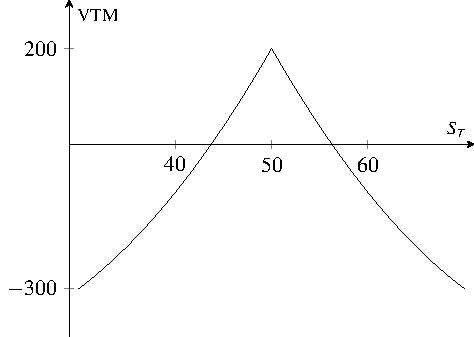
\includegraphics[width=0.7\textwidth]{IMG/Calendar spread at near-term expiration.pdf}
    \label{fig:calendar spreads}
\end{figure}